\chapter{Experimental Framework}
\label{ch:technical}

This chapter describes the experimental framework that supports the empirical work of Chapters~\ref{ch:experimental},~\ref{ch:rq2}, and~\ref{ch:rq3}. Section~\ref{sec:framework-rqs} restates the three research questions in a form that makes explicit what each one measures. Section~\ref{sec:framework-shape-dataset} introduces the shape dataset that all our experiments use, and describes how we generalise it into a Zipfian~\cite{zipf_human_1949} family parametrised by the concentration parameter $\alpha$. Section~\ref{sec:framework-training-setup} covers the training setup: the hyperparameters we keep fixed across all runs, and the computational infrastructure on which the experiments were executed. Section~\ref{sec:framework-validation} reports the validation of the PACE baseline on its original setup, which is a sanity check that our reimplementation reproduces the results of the original paper. The metrics used to evaluate each research question are introduced in the corresponding empirical chapters, where they are actually applied.

\section{Formalisation of the Research Questions}
\label{sec:framework-rqs}

The three research questions introduced in Chapter~\ref{ch:introduction} target three levels at which the input distribution can shape the emergent language. We restate each of them here in a form that makes explicit what we measure and why.

\paragraph*{RQ1: Does the concentration parameter $\alpha$ of the Zipfian input distribution systematically shape the internal structure of the emergent language?}

We measure the internal structure at three levels. First, the total number of abstractions the bandit adopts during training, which tells us how large the emergent vocabulary is. Second, the compression dynamics of the emergent language over the course of training, which we track through the mean length of the messages the speaker produces at each proposal step. Third, the signal that drives adoption: whether the bandit follows the MDL ranking of the candidates it is offered, or their raw frequency in the training data. RQ1 asks whether these three measures depend on $\alpha$ in a systematic way, and whether the dependency is monotone across the range 0.00 to 3.00.

\paragraph*{RQ2: Do populations that share $\alpha$ but differ in ranking develop different abstraction libraries?}

We train twenty PACE populations at each $\alpha$, differing in the ranking permutation used to build the Zipfian dataset. By ranking we mean the specific order in which the 930 training scenes are assigned to positions in the Zipfian distribution: position 1 receives the largest probability mass, position 2 the second largest, and so on. Two populations with the same $\alpha$ but different rankings therefore see the same shape of frequency distribution, but with different specific scenes at each position of the ranking. For each pair of populations, we measure the Jaccard similarity between their adopted abstraction libraries. To interpret the raw overlap values, we compare them to a null model that captures the baseline similarity we would expect by chance under the assumption that abstractions are drawn independently from a shared pool. RQ2 asks whether the observed overlap is systematically different from the null model, whether the difference depends on $\alpha$, and whether the qualitative reasons for divergence can be identified by inspecting the libraries directly.

\paragraph*{RQ3: Do these library-level differences translate into a measurable failure in cross-population communication?}

We test this along three directions. Same-$\alpha$ cross-pairing (Group C in Chapter~\ref{ch:rq3}) pairs agents that share $\alpha$ but differ in ranking, using three distance metrics to select listeners at different notional distances from the speaker. Cross-$\alpha$ pairing (Group X) pairs agents that come from different $\alpha$ values altogether. A third axis (Group O) uses case studies to probe two setups further from the training conditions: a mixed-distribution interaction and an out-of-distribution shift for a single agent. Alongside these, we introduce three modifications to the base same-$\alpha$ setup (Group M) that let us look inside the adaptation dynamics.

RQ3 asks whether adaptation difficulty depends on the distributional distance between the two agents' training conditions, on the concentration regime they share, or on both. The three metrics are designed to distinguish among these alternative hypotheses without pre-empting the conclusion.

\section{The Shape Dataset}
\label{sec:framework-shape-dataset}

All experiments in this thesis use the same underlying task: the one-step signalling game described in Chapter~\ref{ch:pace}. The speaker sees a target scene and, for each action of the program describing that scene, produces a message that the listener combines with its current grid state and the separately supplied positional information to predict the next state. Repeated across the whole sequence of actions, this reconstructs the target. The shapes and scenes come from the dataset introduced in the original PACE paper~\cite{thomas_pace_2025}.

\subsection{Original Construction}
\label{sec:framework-original-construction}

A scene is a configuration of two shapes drawn on a 9-by-9 grid. Each shape is composed of a sequence of primitive actions that place either horizontal or vertical blocks at specific grid positions, and every scene is made from two such shapes placed adjacent to each other on the grid. The full dataset, inherited from PACE~\cite{thomas_pace_2025}, contains 961 scenes, corresponding to all $31 \times 31 = 961$ ordered pairs of the 31 shapes. This gives the dataset a natural two-level structure: at the token level, everything is composed from the two block-placement primitives; at the scene level, the primitives combine into recognisable shapes that then combine into two-shape configurations. The full shape alphabet is shown in Figure~\ref{fig:framework-shape-alphabet}.

\begin{figure}[htbp]
    \centering
    \IfFileExists{images/shape_alphabet.png}{%
        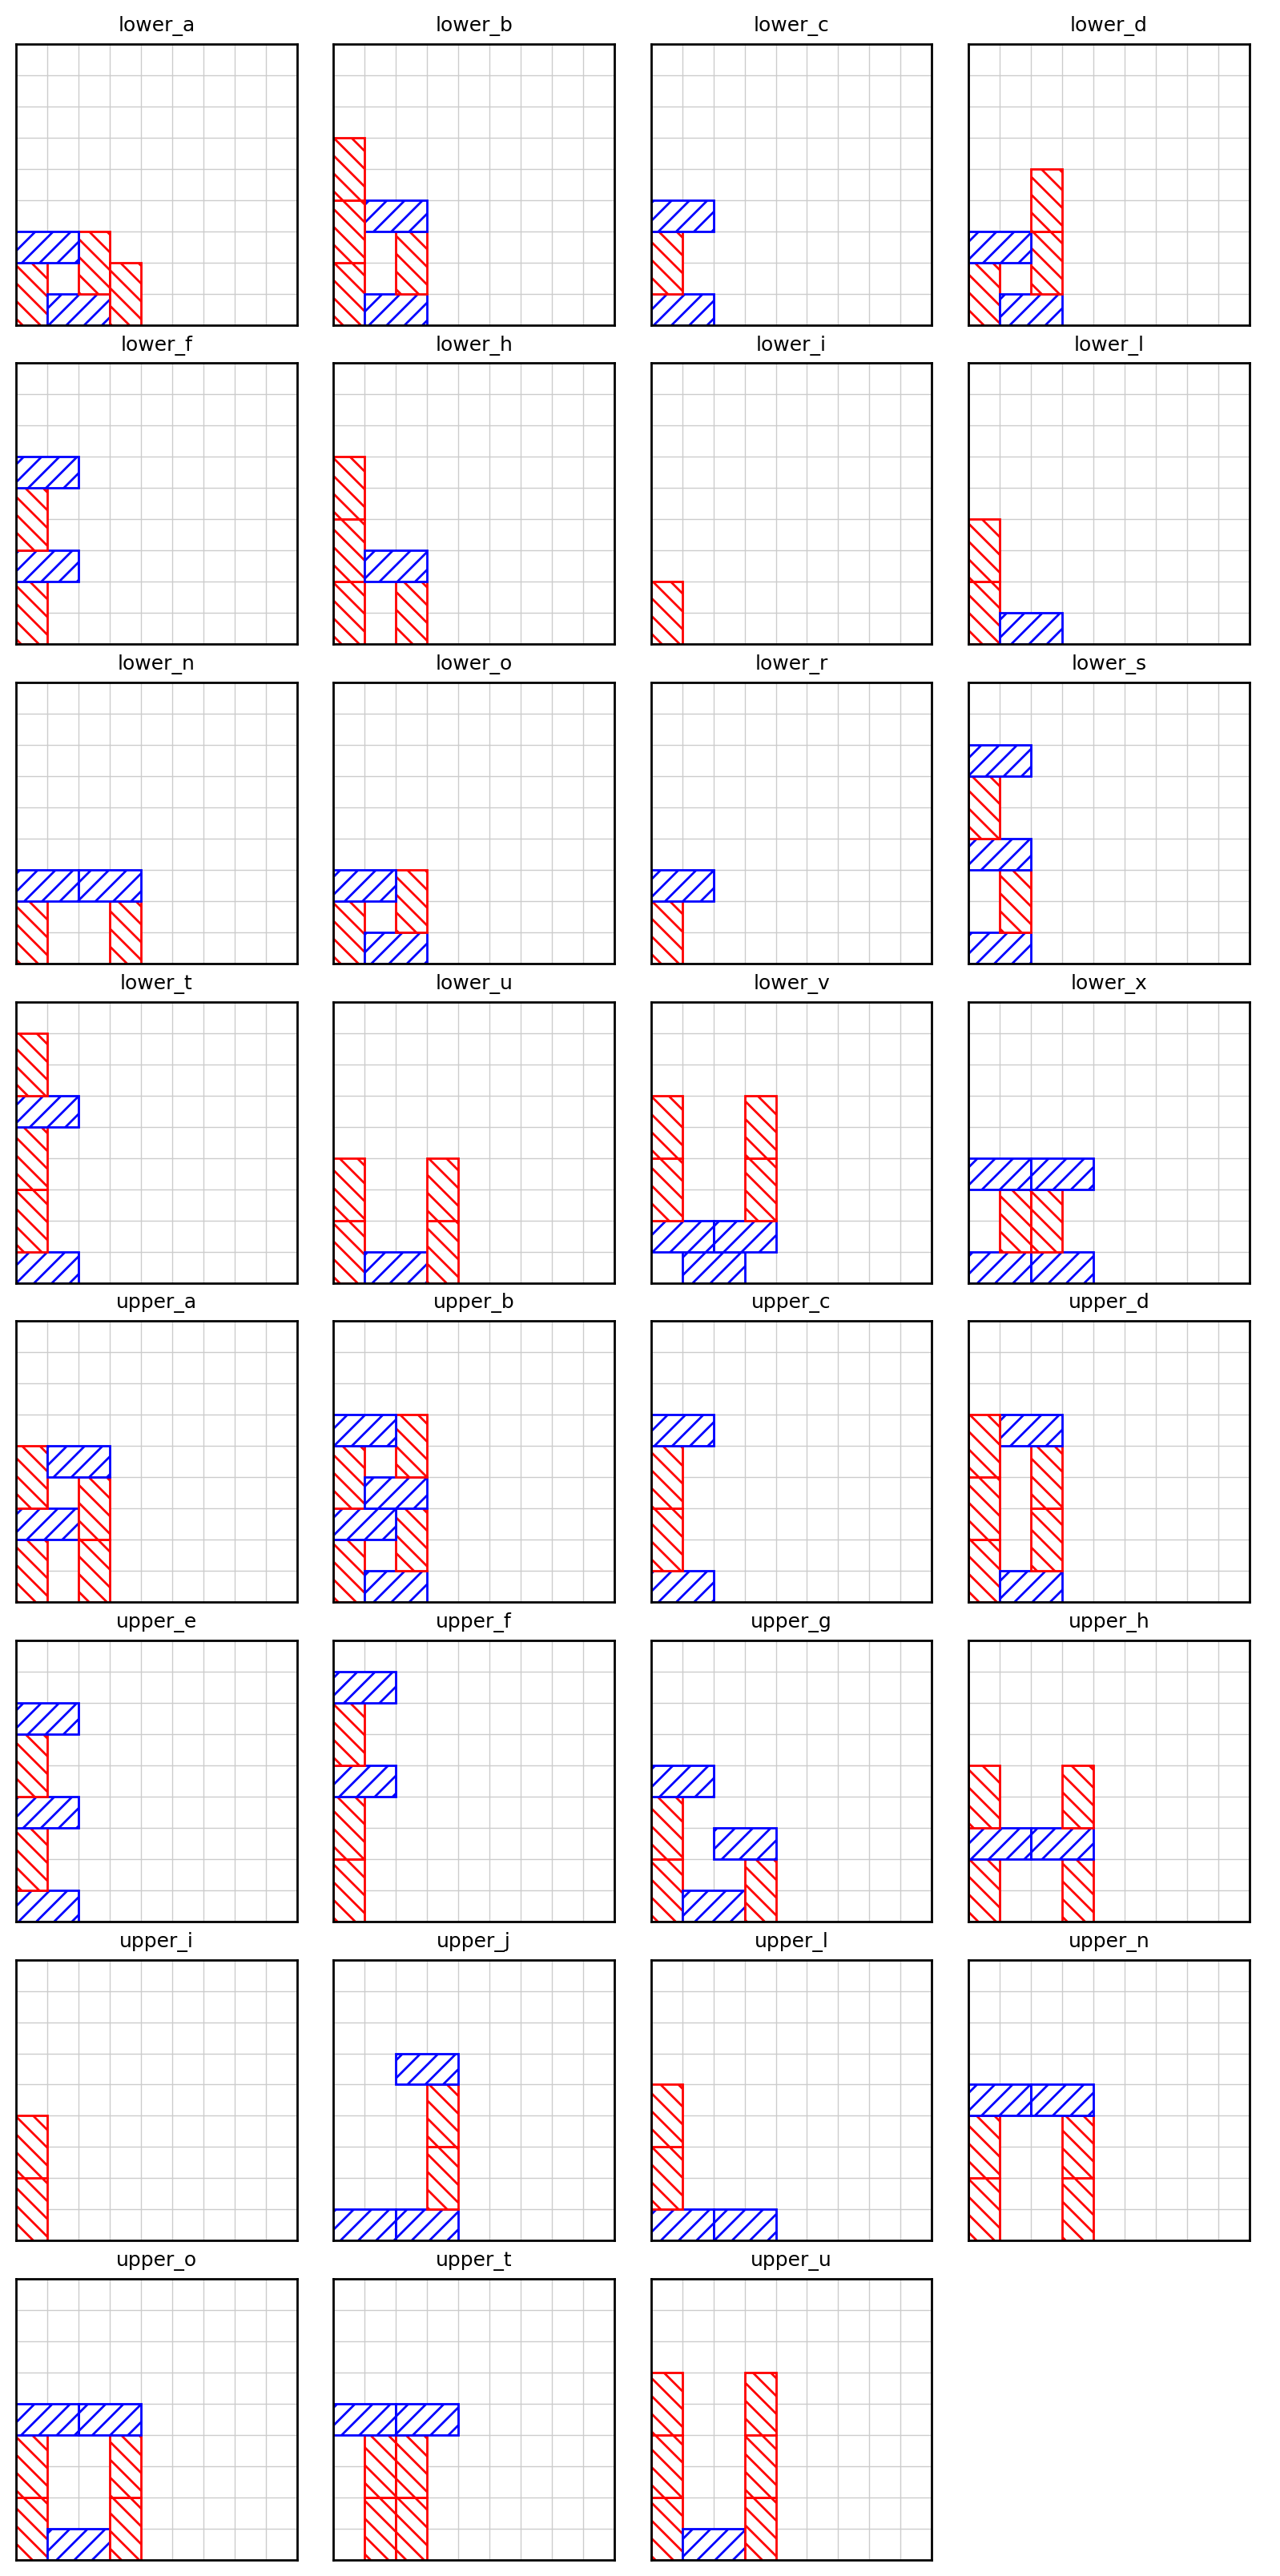
\includegraphics[width=0.78\textwidth]{images/shape_alphabet.png}%
    }{%
        \fcolorbox{red}{white}{\parbox[c][0.14\textheight][c]{0.9\textwidth}{\centering\textcolor{red}{Placeholder figure\\\texttt{\detokenize{images/shape_alphabet.png}}}}}%
    }
    \caption{The 31 shapes that make up the dataset alphabet, each corresponding to an uppercase or lowercase letter and rendered on the 9-by-9 grid. Every shape is built from a sequence of primitive actions placing horizontal or vertical blocks, shown here in the two colours. Scenes are formed by placing two such shapes adjacent to each other, giving all $31 \times 31 = 961$ ordered two-shape configurations.}
    \label{fig:framework-shape-alphabet}
\end{figure}

The speaker's task is to communicate the actions needed to reconstruct the target scene, one at a time; the listener predicts the next grid state from its current state and each message, with positional information supplied separately. In the original PACE setup~\cite{thomas_pace_2025}, the 930 training scenes are sampled uniformly: each has the same probability of being presented during training. This uniform sampling is what we generalise in the next subsection.

\subsection{Zipfian Construction}
\label{sec:framework-zipfian-construction}

To study the effect of input concentration, we generalise the uniform training distribution into a Zipfian family. After separating the 31 held-out test scenes (Section~\ref{sec:framework-data-split}), we apply the Zipfian distribution only to the training set. Given a concentration parameter $\alpha$, we assign the 930 training scenes a probability proportional to $1/k^\alpha$, where $k$ is the rank of the scene in a seed-specific permutation. Higher $\alpha$ means a more concentrated distribution: at $\alpha = 0$ the distribution reduces to uniform sampling, at $\alpha = 3$ the top-ranked scene alone carries roughly 83\% of the training probability mass.

The permutation that determines which scene sits at each rank is drawn once per seed. For a fixed $\alpha$, different seeds produce Zipfian distributions with the same shape but with different scenes at the top of the ranking. This is important for RQ2 and RQ3: two seeds at the same $\alpha$ share the shape of their training distribution but differ in which scenes are frequent. The seed also fixes the neural initialisation of the two agents, so divergence between seeds reflects both sources rather than the ranking difference alone.

We use twenty seeds throughout, listed in Appendix~\ref{ch:apda}. The choice of $\alpha$ values is discussed alongside the specific experiments in the following chapters; for reference, RQ1 uses 21 $\alpha$ values equally spaced between 0.00 and 3.00 in steps of 0.15.

To quantify how far a Zipfian dataset with concentration $\alpha$ departs from the uniform baseline, we compute the Kullback-Leibler (KL) divergence between the two distributions. KL divergence~\cite{cover_elements_2006} measures how much information is lost when the uniform distribution is used to approximate the Zipfian one, and takes value zero when the two distributions coincide. For our datasets, KL is zero at $\alpha = 0$ by construction, grows steadily through the intermediate range, and reaches substantial values at the top of the $\alpha$ range. The KL divergence suits this comparison because it is asymmetric in a way that reflects the direction of the deviation. It grows when the Zipfian distribution concentrates mass on scenes that the uniform baseline treats as one of many, but it does not grow further if additional scenes have zero probability under the Zipfian. This asymmetry is what makes it a natural measure of concentration. The KL divergence between each $\alpha$ and the uniform baseline is also used later, in Chapter~\ref{ch:rq3}, as one of three metrics to characterise the distributional distance between two populations trained on different concentration parameters. Per-$\alpha$ snapshots of the underlying subsequence distributions are reported in Appendix~\ref{ch:apdd}.

The KL divergence is not the only way to quantify how concentrated a Zipfian dataset is. Several classical measures of statistical concentration apply equally well to the pair frequency distribution, and we report four of them in Appendix~\ref{ch:apdd}. Shannon entropy quantifies the total uncertainty in the distribution, and is high when the mass is spread over many pairs at comparable frequencies. Simpson diversity measures the probability that two randomly drawn pair occurrences correspond to different pairs, and is maximal under uniform sampling. The Gini coefficient reports the aggregate inequality of the distribution, from zero when all pairs are equally frequent to values close to one when a small subset dominates. The imbalance ratio divides the frequency of the most common pair by that of the least common one, and is the most sensitive of the four to the tail of the distribution. All four move with $\alpha$ in the direction the Zipfian construction intends, confirming that concentration grows as designed; the values are reported in Appendix~\ref{ch:apdd}.

To give a concrete visual sense of what the concentration parameter $\alpha$ does to the training data, Figures~\ref{fig:framework-primitive-patterns-alpha-000} and~\ref{fig:framework-primitive-patterns-alpha-300} show the frequency distribution of primitive subsequences in two representative datasets: one with uniform sampling ($\alpha = 0.00$) and one with strong concentration ($\alpha = 3.00$). Each bar corresponds to a distinct subsequence, and the bar height reports how often that subsequence appears in the training set. At $\alpha = 0.00$, the distribution is broad and comparatively flat: many subsequences appear at similar frequencies, and there is no clear dominance of any specific pattern. At $\alpha = 3.00$, the distribution is sharply concentrated: a small number of subsequences account for the bulk of the training exposures, while the majority appear rarely or not at all. Both figures use the same seed (seed 42), so the identity of the subsequences at each rank is comparable across the two plots; what changes is only the concentration profile assigned by $\alpha$.

\begin{figure}[htbp]
    \centering
    \IfFileExists{images/primitive_patterns_alpha_0.00.png}{%
        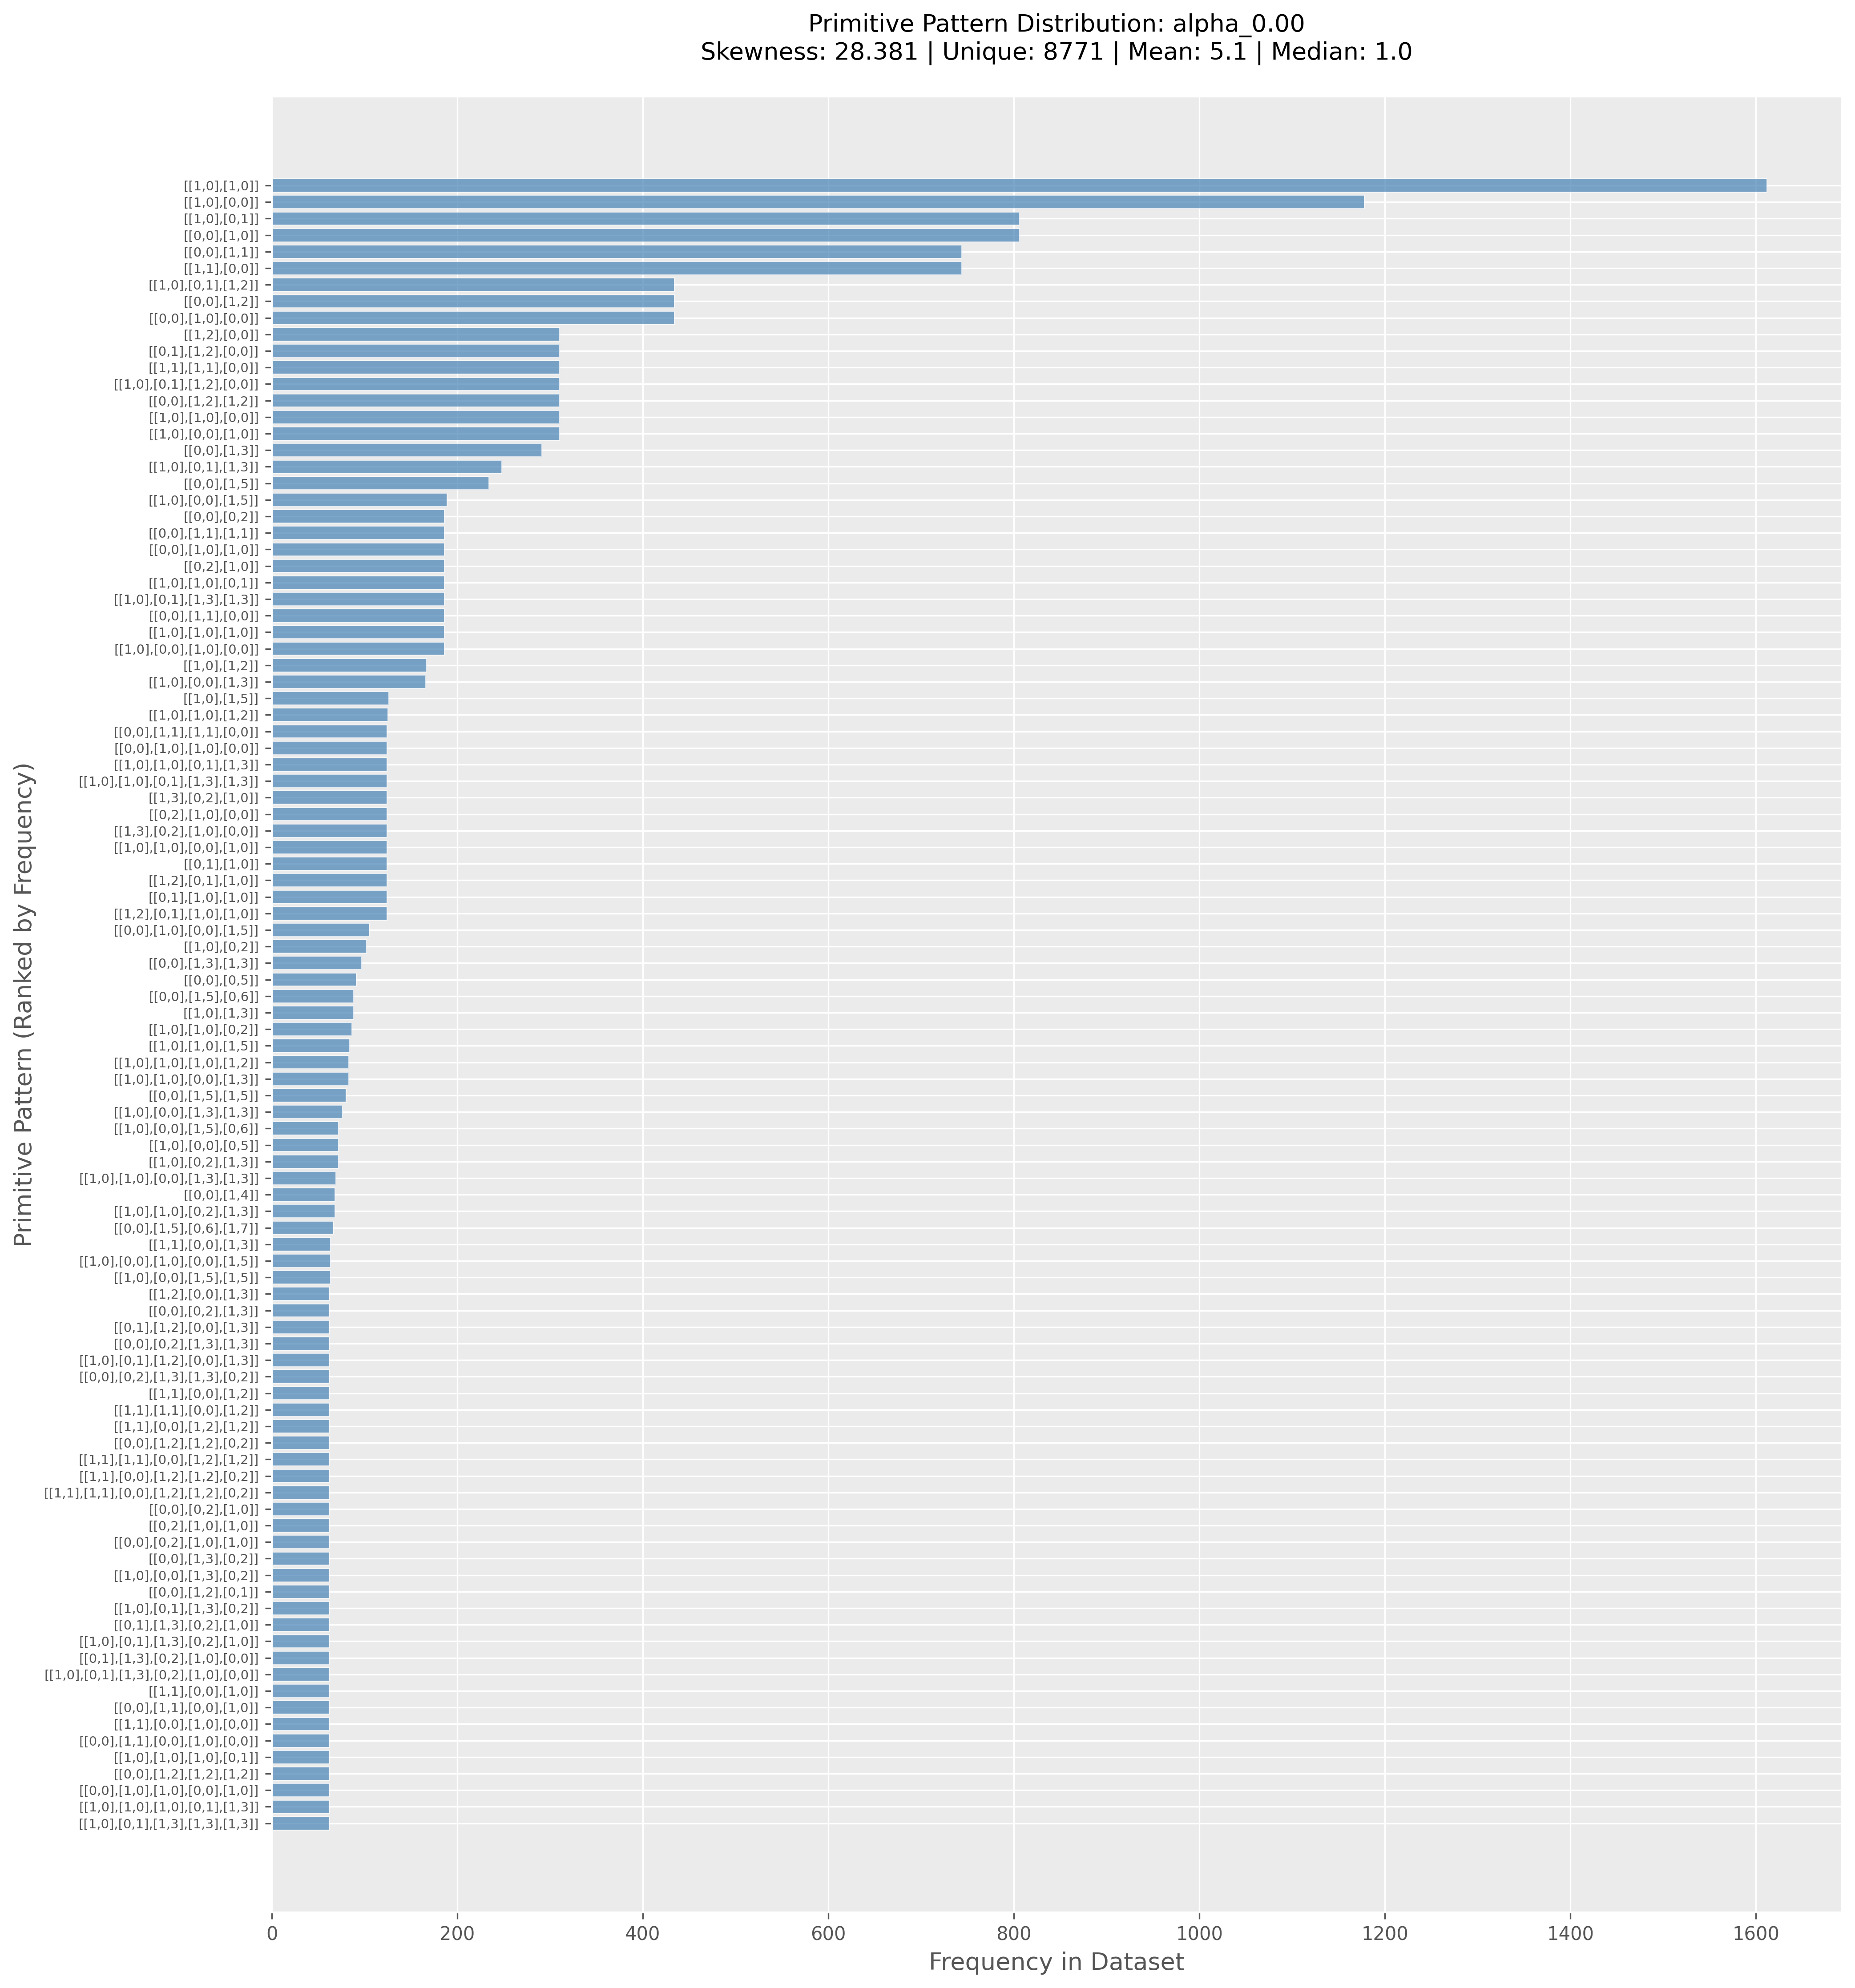
\includegraphics[width=0.95\textwidth]{images/primitive_patterns_alpha_0.00.png}%
    }{%
        \fcolorbox{red}{white}{\parbox[c][0.14\textheight][c]{0.9\textwidth}{\centering\textcolor{red}{Placeholder figure\\\texttt{\detokenize{images/primitive_patterns_alpha_0.00.png}}}}}%
    }
    \caption{Frequency distribution of primitive subsequences in the training dataset at $\alpha = 0.00$ (uniform sampling), seed 42. Each bar shows one subsequence's raw frequency across the 930 training scenes.}
    \label{fig:framework-primitive-patterns-alpha-000}
\end{figure}

\begin{figure}[htbp]
    \centering
    \IfFileExists{images/primitive_patterns_alpha_3.00.png}{%
        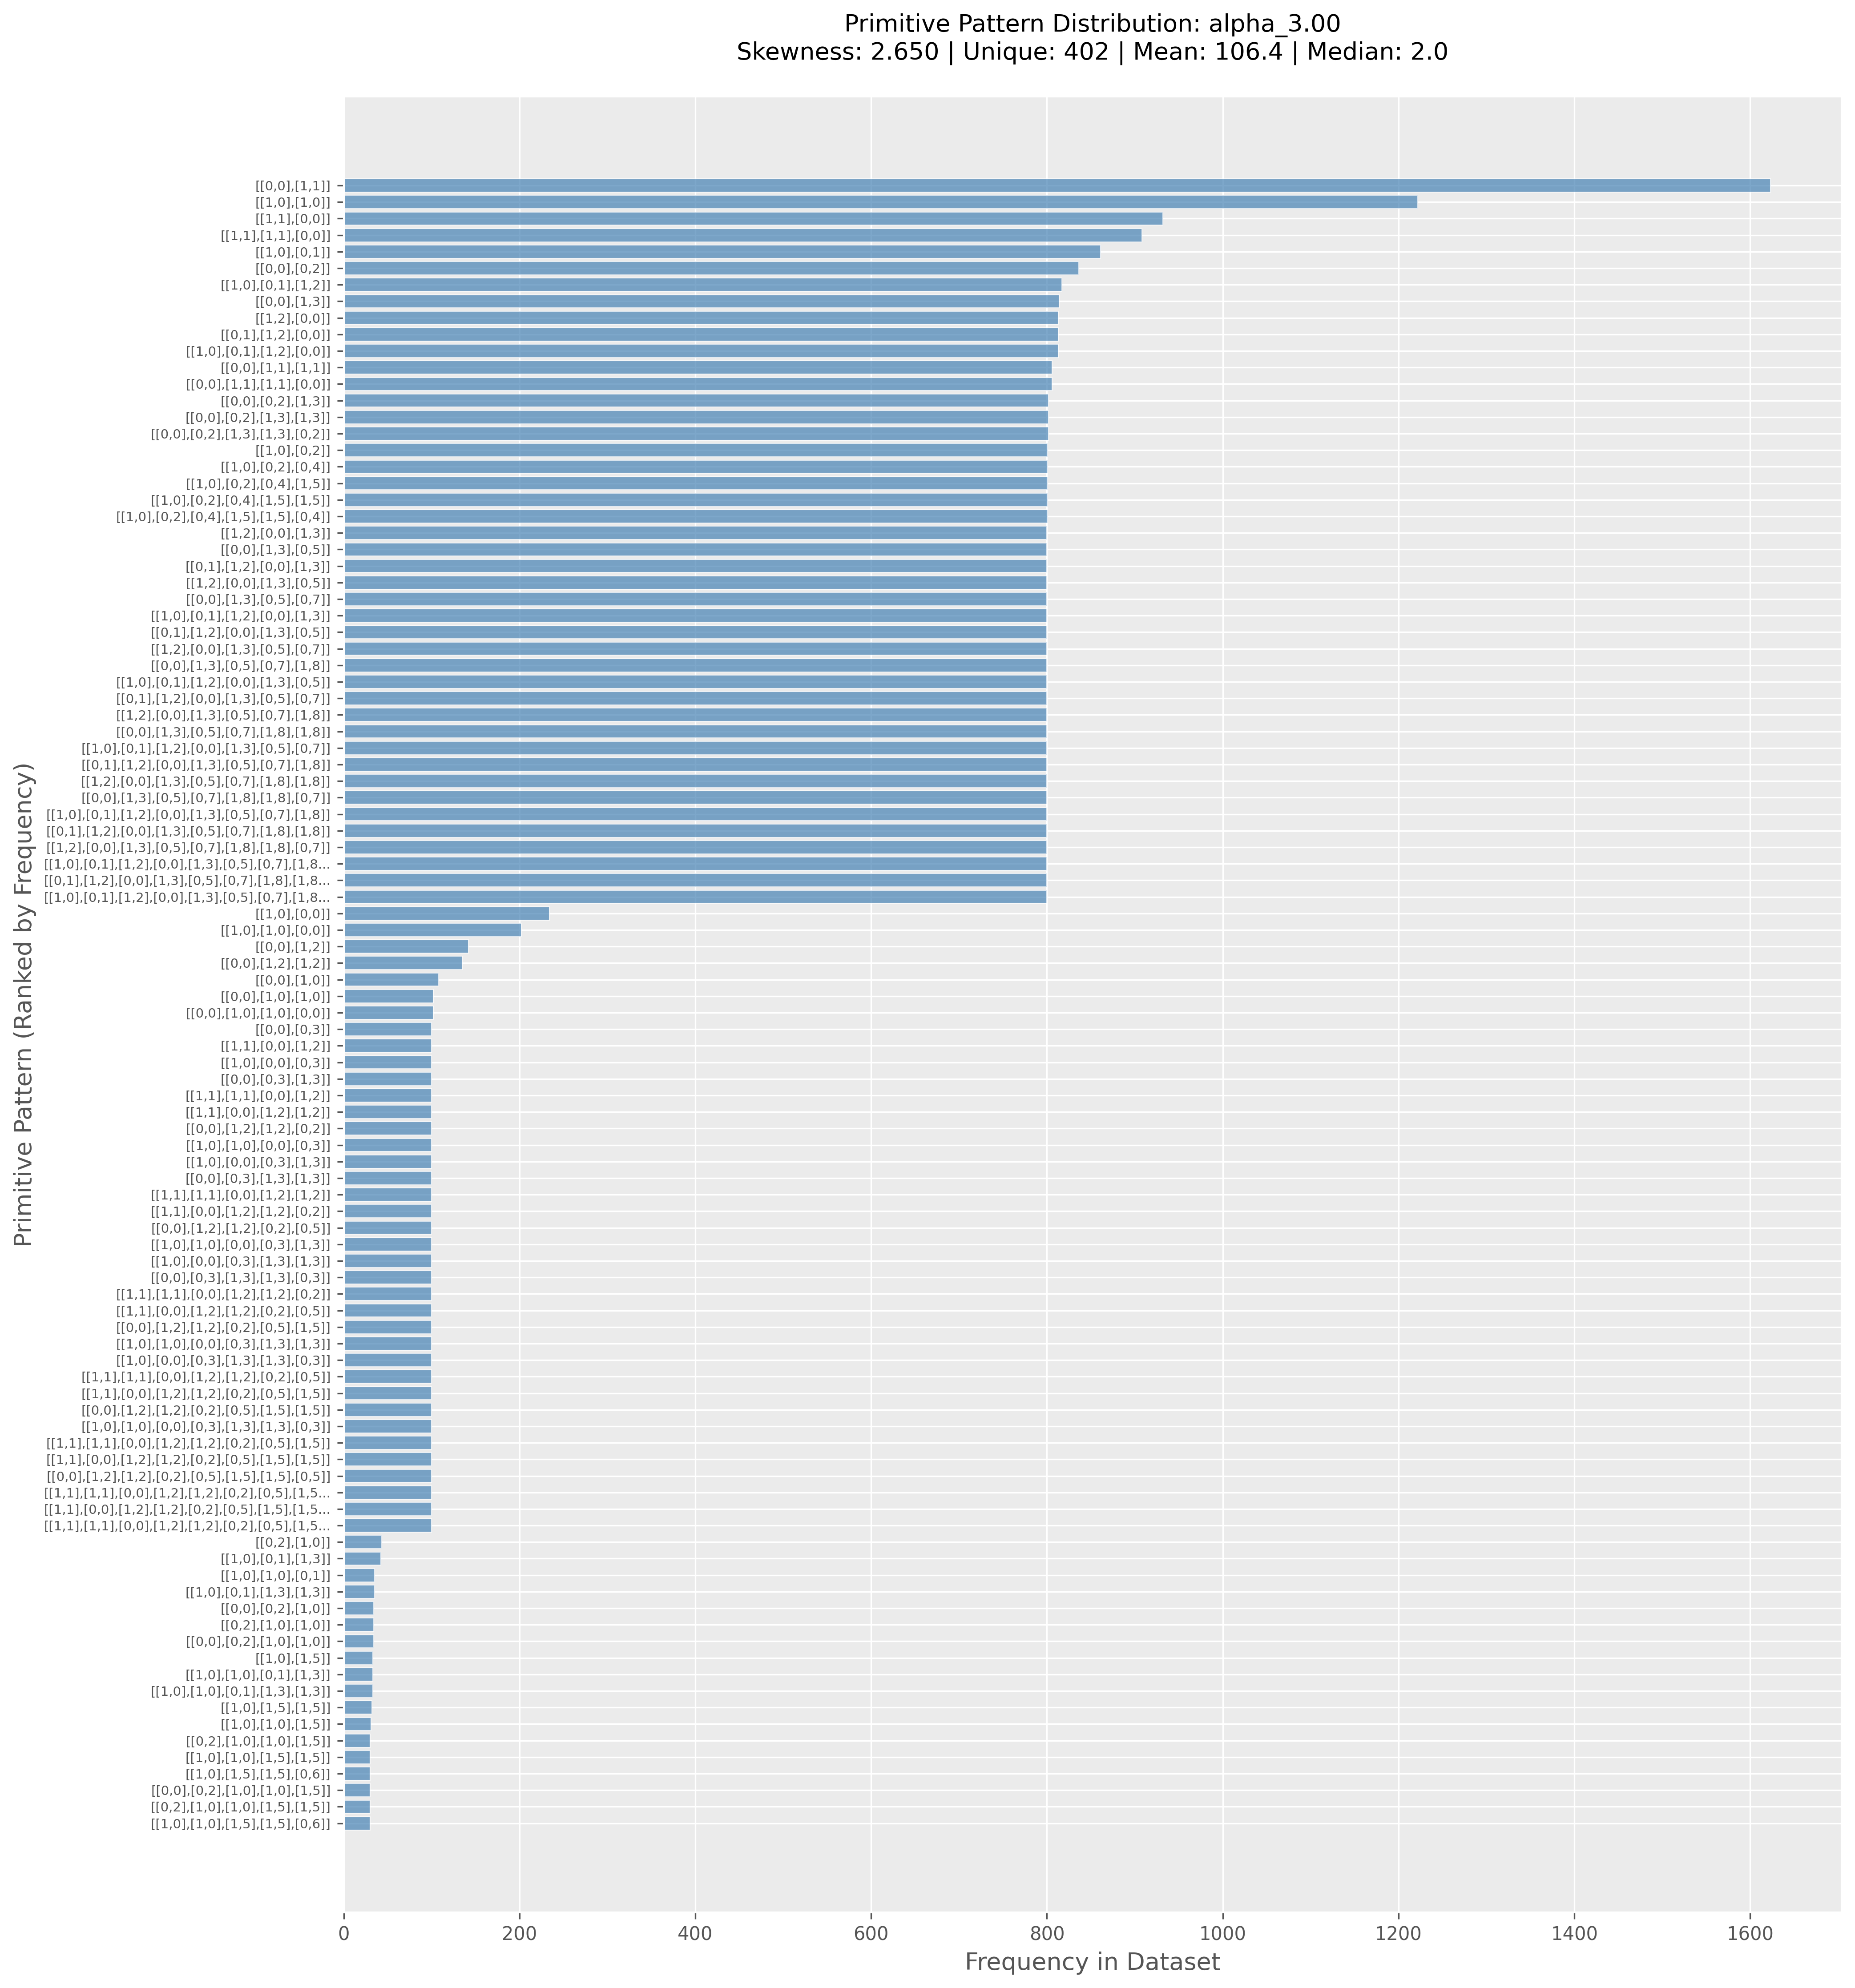
\includegraphics[width=0.95\textwidth]{images/primitive_patterns_alpha_3.00.png}%
    }{%
        \fcolorbox{red}{white}{\parbox[c][0.14\textheight][c]{0.9\textwidth}{\centering\textcolor{red}{Placeholder figure\\\texttt{\detokenize{images/primitive_patterns_alpha_3.00.png}}}}}%
    }
    \caption{Same as Figure~\ref{fig:framework-primitive-patterns-alpha-000} but at $\alpha = 3.00$ (strong concentration), seed 42. The distribution is visibly sharper, with a small number of subsequences dominating.}
    \label{fig:framework-primitive-patterns-alpha-300}
\end{figure}

\subsection{Data Split}
\label{sec:framework-data-split}

For every dataset (seed and $\alpha$ combination), we use the original PACE split~\cite{thomas_pace_2025}: 930 scenes for training and 31 held-out scenes for testing. The 31 test scenes are excluded from the Zipfian ranking and training-frequency assignment. The test set is used to evaluate reconstruction accuracy at every training epoch, and all test evaluations reported in this thesis are on this held-out set.

\section{Training Setup}
\label{sec:framework-training-setup}

\paragraph{Training setup.}
We train each PACE agent for $s = 20$ Abstraction phases, each preceded by $e = 40$ Communication epochs. During each Communication epoch, the bandit selects a program for each scene, and the neural agents are updated by mini-batch gradient descent on the reconstruction loss described in Section~\ref{sec:pace-communication}. Reconstruction rewards update the bandit as described in Section~\ref{sec:pace-selection}. Each Abstraction phase introduces a new token using the MDL-based procedure described in Section~\ref{sec:pace-abstraction}.

The full list of hyperparameters (learning rate, batch size, hidden layer sizes, Gumbel-softmax temperature, bandit $\varepsilon$, MDL cutoff) is reported in Appendix~\ref{ch:apdb}. As explained in Section~\ref{sec:pace-extensions}, these values are fixed across all runs and conditions so that the experimental variation comes from the training distribution rather than from implicit per-condition tuning. The values are the ones used in the original PACE paper~\cite{thomas_pace_2025} wherever they were specified.

\paragraph{Hardware and compute.}
The experimental campaign was run on the C3SE Vera cluster. As discussed in Appendix~\ref{ch:apda}, the available compute budget determined the choice of twenty seeds across 21 concentration values, giving 420 main training runs.

\section{Validation of PACE on the Original Setup}
\label{sec:framework-validation}

Before running any of the Zipfian experiments, we validate the reimplementation of PACE we use throughout this thesis against the original paper's setup~\cite{thomas_pace_2025}. The validation is a sanity check that the system trains and behaves as expected before we start modifying its training distribution.

We evaluate PACE, Greedy, and No abstractions on the original uniform training distribution ($\alpha = 0.00$), using the hyperparameters from the original paper. The validation compares program-length and held-out reconstruction-accuracy trajectories, and also records the number of adopted abstractions. The configurations reproduce the qualitative contrast between compression and accuracy; the numerical results and their comparison with the original paper are reported in Appendix~\ref{ch:apdc}. This check supports using the implementation for the subsequent experiments, without claiming an exact numerical reproduction.